\chapter{Introduction}

The ecoMOD project is focused on creating sustainable, prefabricated housing units in partnership with local affordable housing organizations. These units are sustainable in that are environmentally responsive, with reduced energy, water, and maintenance costs compared to traditional housing stock. ecoMOD housing is aggressively affordable without cutting corners in construction, and strives to utilize the latest best practices in green, low-impact building and construction for a total cost of ownership that is markedly less than average. As a result, ecoOMOD housing has received numerous awards and accolades in the trade space\cite{Lau2013}.

\begin{figure}
\centering
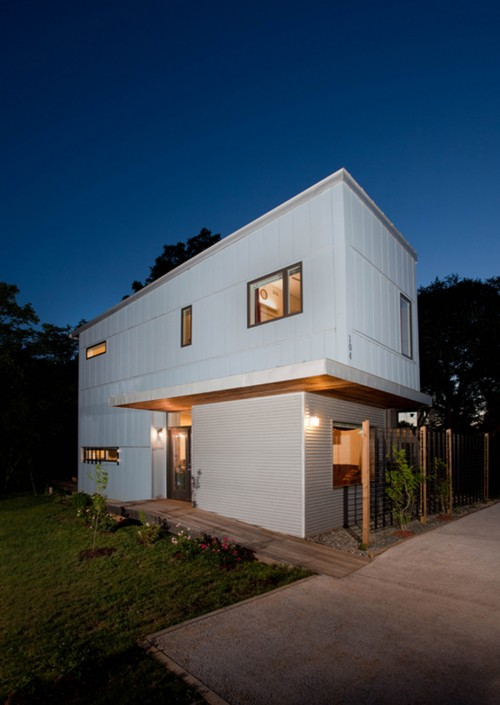
\includegraphics[width=0.3\linewidth]{./images/SFSmith_110602_8113-copy-500x705}
\caption{ecoMOD 4 in the evening\cite{Smith2011}}
\label{fig:SFSmith_110602_8113-copy-500x705}
\end{figure}

Historically, all ecoMOD housing has been extensively monitored with electronic instrumentation and networked for reasons of evaluating building performance. These sensors monitor important information such as ambient temperature, humidity levels, air quality, and electricity use. Data is collected and sent back to the University of Virginia for analysis. Residential buildings account for more than a third of total power consumption use (excluding transportation) in the United States\cite{EIA2015}. Quantifying the benefit of various design selections and operational behaviors is critical to analyzing the costs and benefits, and is the only way to provide targeted, effective feedback on methods of reducing construction cost and energy consumption.

Existing commercial monitoring solutions usually suffer the following problem: either they are excessively costly to install in the field, or are unreliable and difficult to integrate into existing data retrieval schemes. The ecoMOD project is no stranger to sensor deployments, having previously successfully opted to use expensive commercial solutions from vendors such as National Instruments or Onset Computers. Despite the cost, systems like the ones from National Instruments are being deployed year-after-year in many different buildings. They have seen extensive use in the commercial building industry due to the greater amount of capital and land involved. This demonstrates the clear value proposition of environmental monitoring systems. If these systems could be made cheaper, more accurate, and easier to use, homeowners and renters could objectively assess and audit their building performance metrics.

In this thesis, the design of a new sensing platform is presented. It is an extension of monitoring work that has been done continuously since the inception of the project, while introducing the foundations for future work in enabling environmental control by increasing platform capability. It is an evolutionary improvement over previous work done by Ernest Bowden in developing a development platform based around the MSP430 for the ecoMOD project\cite{Bowden2009}. The design was conducted with three major goals compared to previous work: easier deployments, increased robustness for experimentation, and retaining a low power consumption envelope. The designed node accomplishes this through three methods: use of 802.11 and Internet communication protocols for deployability, increased microprocessor speed and memory, and a very aggressive sleep schedule combined with a responsive, event-based software framework.

\section{Related Work}

As mentioned previously, commercial sensor deployments from vendors such as National Instruments (NI) were used to instrument the first ecoMOD housing iterations\cite{Kidd2007}. However, as a business-focused product, the NI system was extremely expensive, with a small sensor deployment costing over \$10,000. Subsequent ecoMOD installations used a mixture of purpose-built electronics together with commercial-off-the-shelf (COTS) systems for monitoring. These included systems such as The Energy Detective (TED) from Energy Inc. (2009), and the Vantage Vue weather station from Davis Instruments. In general, this approach worked, but separate sensors were difficult to integrate into a whole sensing and monitoring system, as each device had its own unique interface and controls.

Failure to inter-operate is a well-known limitation of existing sensor network deployments. Commercially available devices use incompatible physical and application layer interfaces. At the physical and associated low communication layers, the most popular of these include IEEE 802.15.4, Bluetooth Low-energy, and IEEE 802.11. At the application layer, Zigbee, Z-Wave, WirelessHART, and the Constrained Application Protocol (CoAP) all enjoy significant mindshare. While there has been a push from industry players towards standardization of application and physical layer protocols, the market remains fragmented and many vendors lock customers in with proprietary, incompatible, and undocumented interfaces.

As the capabilities of microcontrollers increase, new choices in communication protocals become feasible. For a great deal of time, Internet Protocol (IP) was not used because it was considered inappropriate for use in embedded wireless sensor networks. Traditional mobile WiFi chips were targeted at laptops and cell-phones, which needed to be recharged on a daily or hourly basis. In addition, the protocol required too many computing resources as a proportion of microcontroller capability, especially at WiFi's higher data rates and encryption complexities. However, the problem has been solved from two sides. First, the steady advance of Moore's Law has brought down the cost in power and money of embedding computing capability. Second, the IETF has defined several reduced-functionality subsets of certain IP or IP-related protocols that can be implemented on resource-constrained computers, e.g. 6LowPAN\cite{Montenegro2007}, RoLL\cite{Winter2012}, CoAP\cite{Z.Shelby2014}. The usage of Internet protocols has even been adopted by the ZigBee Alliance (an industry association of electronics manufacturers) in their "ZigBee IP" networking specification.

The device designed in this thesis utilizes a full 802.11-compatible communication stack along with an  hypertext transport protocol (HTTP) interface. The adoption of IP/HTTP for wireless sensor networks will speed their deployment and adoption. Communication compatibility between disparate devices will enable more competition between manufacturers, lower costs, and facilitate the creation of new services which span multiple sensor deployments. It will also allow the easy use of well-known Web technologies for aggregating and displaying sensor information.

\begin{figure}[h]
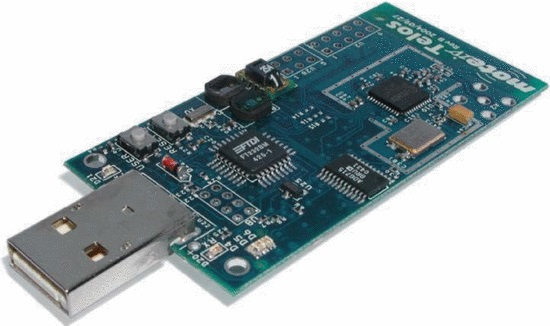
\includegraphics[width=0.4\textwidth]{images/telosb}
\caption{TelosB Sensor Mote\cite{Polastre2005}}
\label{telosB}
\end{figure}

Residential environmental monitoring can be considered a subset of the broader networked sensor market. In academic wireless sensor network (WSN) research, a sensor node is popularly known as a "mote", which comes from the idea that future sensor nodes will be as ubiquitous as dust motes in an Internet cloud of devices. These existing devices have been used for many years to investigate new networking techniques and to collect data for environmental monitoring. As a result, the explored design space is similar to what is designed in this thesis. 

There are many commercially available motes. Interest in distributed sensing has only increased with the ongoing media coverage of the possibilities of the "Internet of Things", which is the idea that all future electronic devices will be seamlessly interconnected via the Internet due to rapidly declining costs in wireless technology. It is thought that by easily enabling the collection of data from large numbers of different sensors, new conclusions and insights can be drawn from the number of data correlations that can be formed. For example, suppose we have pervasive independent light, temperature, and sound sensors in a home. By correlating their observations, it is possible that home occupancy could be sensed on a per-room basis, even with a sparse sensor placement strategy.

Typical mote characteristics are described in Table \ref{mote_characteristics}. Generally, they include several default sensors, a low-power transceiver, an 8-bit microcontroller, and tens of kilobytes of code data and storage. As development boards they have many pins broken out for easy expandability. While bare-metal programming of these devices is popular, two operating systems exist for these platforms, where new networking and application layer protocols are tested and researched. These are Berkeley's TinyOS\cite{Levis2005}, and the Swedish Institute of Computer Science's (SICS) ContikiOS\cite{Dunkels2011}. 

\begin{table}[h]
\begin{tabular}{@{}lllll@{}}
\toprule
Processor & Platform Name & Speed (MHz) & Ram (Kb) & Transceiver \\ \midrule
TI MSP430 & TelosB & 8 & 10 & TI CC2420 \\
Atmel ATMega 128l & MicaZ & 8 & 4 & TI CC2420 \\
MC1322x & Econotag & 26 & 128 & MC1322x \\
Atmel ATMega 128 & Waspmote & 14 & 8 & Varies \\ \bottomrule
\end{tabular}
\caption{Typical Mote Characteristics}
\label{mote_characteristics}
\end{table}

Perhaps the most popular mote for sensor network research over the past decade has been the Mica-series from MEMSIC Inc. The initial Mica platform was released in 2001\cite{hill2002mica}, with the latest Mica release named the MicaZ. Despite the many years in between, the MicaZ is similar in capabilities to the original Mica, differing only in the radio on-board. The trend in mote development has been to hold microcontroller resources constant, while decreasing per unit cost. The defining feature of the research in this area has been in the adaptations necessary for computations on limited and resource-constrained devices. 

\section{Contributions}

This thesis describes a method for designing a development platform that allows for further research and monitoring into building performance envelopes. Power consumption is analyzed, and various methods for extending battery lifetime are explored. Chapter 1 explores the hardware design choices: power supplies, microprocessor choices, sensor suites, and communication possibilities. Chapter 2 does a similar exploration of the various choices that can be made for firmware load, along with application layer communication choices. Chapter 3 presents a short overview of various energy trade-offs, followed by Chapter 4, which contains a conclusion and a summary of further work. The appendix contains the circuit board schematics as well as the bill of materials. 